\section{Theorie}
\subsection{Widerstandsmessung}
Im Allgemeinen idealen Fall lassen sich Widerstände simpel über das Ohmsche Gesetz $ R = \frac{U}{I} $ berechnen. Näherungsweise lässt sich diese Formel auch für niedrige Widerstände verwenden, geht man aber zu größeren Widerständen, wie etwa bei diesem Experiment über, werden die Störfaktoren wie der Innenwiderstand relevanter, sodass man alternative Messmethoden braucht. Eine weitere, genauere Methode bietet die Wheatstonesche Brückenschaltung, bei der man das Problem des Innenwiderstandes überwindet, wir betrachten bei unserem Experiment aber die Ladungen in einem $ R $-$ C $-Parallelschwingkreis. Hierbei ist die Formel für die Entladung eines Kondensators:
\begin{align}
Q(t) & = Q_0 \cdot e^{- \frac{t}{R \cdot C}}
\end{align}
Für die Messung zu verschiedenen Zeiten $t_1$, $t_2$ gilt:
\begin{align}
\frac{Q(t_1)}{Q(t_2)} & = e^{\frac{t_2 - t_1}{R \cdot C}} \\
\Leftrightarrow R & = \frac{t_2 - t_1}{C \cdot \ln{ \frac{Q(t_1)}{Q(t_2)}}} \text{.}
\end{align}
Diese Formel ist nur bei hohen Widerständen genau, da der Kondensator sich sonst zu schnell entläd und man keine genauen Ladungswiderstände messen kann.
\subsection{Ladungsmessung}
Zur Ladungsmessung verwenden wir einen Stromintegrator
\subsection{$R$-$L$- und $R$-$L$-$C$-Parallelschwingkreis}
%\begin{minipage}{5cm}
%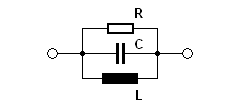
\includegraphics{RLC-Schwingkreis.png}
%\end{minipage}
Beim $ R $-$ L $-$ C $-Parallelschwingkreis handelt es sich um eine Parallelschaltung von Widerstand $ R $, Spule $ L $ und Kondensator $ C $. Über die Kirchhoffsche Maschenregel, in diesem Fall $ \sum_i I_i = 0 $ stößt man für die Ladung auf eine lineare, homogene Differentialgleichung 2. Ordnung der Form
\begin{align}
\ddot{Q} + 2 \beta \dot{Q} + \omega_{0}^2 Q = 0 \text{,}
\end{align}
wobei $ \beta : = \frac{R}{2L} $ und $ \omega_{0} : = \sqrt{ \frac{1}{LC}} $ ist.

\subsection{Bestimmung der elektrischen Feldkonstante}
Mithilfe des Kirchhoffschen Gesetzes ergibt sich für die Kapazität $C$ des Plattenkondensators (Plattenabstand $d$, -radius $r$, -anzahl $n$)
\begin{align}
C&=\varepsilon_0\varepsilon_r\*(n-1)\*\left(\frac{\pi r^2}{d}+r\*\left(\ln{\left(\frac{16\pi r}{d}\right)}-1\right)\right)
\end{align}
Kennt man nun die Kapazität $C$ des Kondensators, lässt sich die elektrische Feldkonstante $\varepsilon_0$